% Options for packages loaded elsewhere
\PassOptionsToPackage{unicode}{hyperref}
\PassOptionsToPackage{hyphens}{url}
\PassOptionsToPackage{dvipsnames,svgnames,x11names}{xcolor}
%
\documentclass[
  a4paperpaper,
]{article}

\usepackage{amsmath,amssymb}
\usepackage{iftex}
\ifPDFTeX
  \usepackage[T1]{fontenc}
  \usepackage[utf8]{inputenc}
  \usepackage{textcomp} % provide euro and other symbols
\else % if luatex or xetex
  \ifXeTeX
    \usepackage{mathspec} % this also loads fontspec
  \else
    \usepackage{unicode-math} % this also loads fontspec
  \fi
  \defaultfontfeatures{Scale=MatchLowercase}
  \defaultfontfeatures[\rmfamily]{Ligatures=TeX,Scale=1}
\fi
\usepackage{lmodern}
\ifPDFTeX\else  
    % xetex/luatex font selection
\fi
% Use upquote if available, for straight quotes in verbatim environments
\IfFileExists{upquote.sty}{\usepackage{upquote}}{}
\IfFileExists{microtype.sty}{% use microtype if available
  \usepackage[]{microtype}
  \UseMicrotypeSet[protrusion]{basicmath} % disable protrusion for tt fonts
}{}
\makeatletter
\@ifundefined{KOMAClassName}{% if non-KOMA class
  \IfFileExists{parskip.sty}{%
    \usepackage{parskip}
  }{% else
    \setlength{\parindent}{0pt}
    \setlength{\parskip}{6pt plus 2pt minus 1pt}}
}{% if KOMA class
  \KOMAoptions{parskip=half}}
\makeatother
\usepackage{xcolor}
\usepackage[top=30mm,left=30mm,right=30mm,heightrounded]{geometry}
\setlength{\emergencystretch}{3em} % prevent overfull lines
\setcounter{secnumdepth}{-\maxdimen} % remove section numbering
% Make \paragraph and \subparagraph free-standing
\ifx\paragraph\undefined\else
  \let\oldparagraph\paragraph
  \renewcommand{\paragraph}[1]{\oldparagraph{#1}\mbox{}}
\fi
\ifx\subparagraph\undefined\else
  \let\oldsubparagraph\subparagraph
  \renewcommand{\subparagraph}[1]{\oldsubparagraph{#1}\mbox{}}
\fi

\usepackage{color}
\usepackage{fancyvrb}
\newcommand{\VerbBar}{|}
\newcommand{\VERB}{\Verb[commandchars=\\\{\}]}
\DefineVerbatimEnvironment{Highlighting}{Verbatim}{commandchars=\\\{\}}
% Add ',fontsize=\small' for more characters per line
\usepackage{framed}
\definecolor{shadecolor}{RGB}{241,243,245}
\newenvironment{Shaded}{\begin{snugshade}}{\end{snugshade}}
\newcommand{\AlertTok}[1]{\textcolor[rgb]{0.68,0.00,0.00}{#1}}
\newcommand{\AnnotationTok}[1]{\textcolor[rgb]{0.37,0.37,0.37}{#1}}
\newcommand{\AttributeTok}[1]{\textcolor[rgb]{0.40,0.45,0.13}{#1}}
\newcommand{\BaseNTok}[1]{\textcolor[rgb]{0.68,0.00,0.00}{#1}}
\newcommand{\BuiltInTok}[1]{\textcolor[rgb]{0.00,0.23,0.31}{#1}}
\newcommand{\CharTok}[1]{\textcolor[rgb]{0.13,0.47,0.30}{#1}}
\newcommand{\CommentTok}[1]{\textcolor[rgb]{0.37,0.37,0.37}{#1}}
\newcommand{\CommentVarTok}[1]{\textcolor[rgb]{0.37,0.37,0.37}{\textit{#1}}}
\newcommand{\ConstantTok}[1]{\textcolor[rgb]{0.56,0.35,0.01}{#1}}
\newcommand{\ControlFlowTok}[1]{\textcolor[rgb]{0.00,0.23,0.31}{#1}}
\newcommand{\DataTypeTok}[1]{\textcolor[rgb]{0.68,0.00,0.00}{#1}}
\newcommand{\DecValTok}[1]{\textcolor[rgb]{0.68,0.00,0.00}{#1}}
\newcommand{\DocumentationTok}[1]{\textcolor[rgb]{0.37,0.37,0.37}{\textit{#1}}}
\newcommand{\ErrorTok}[1]{\textcolor[rgb]{0.68,0.00,0.00}{#1}}
\newcommand{\ExtensionTok}[1]{\textcolor[rgb]{0.00,0.23,0.31}{#1}}
\newcommand{\FloatTok}[1]{\textcolor[rgb]{0.68,0.00,0.00}{#1}}
\newcommand{\FunctionTok}[1]{\textcolor[rgb]{0.28,0.35,0.67}{#1}}
\newcommand{\ImportTok}[1]{\textcolor[rgb]{0.00,0.46,0.62}{#1}}
\newcommand{\InformationTok}[1]{\textcolor[rgb]{0.37,0.37,0.37}{#1}}
\newcommand{\KeywordTok}[1]{\textcolor[rgb]{0.00,0.23,0.31}{#1}}
\newcommand{\NormalTok}[1]{\textcolor[rgb]{0.00,0.23,0.31}{#1}}
\newcommand{\OperatorTok}[1]{\textcolor[rgb]{0.37,0.37,0.37}{#1}}
\newcommand{\OtherTok}[1]{\textcolor[rgb]{0.00,0.23,0.31}{#1}}
\newcommand{\PreprocessorTok}[1]{\textcolor[rgb]{0.68,0.00,0.00}{#1}}
\newcommand{\RegionMarkerTok}[1]{\textcolor[rgb]{0.00,0.23,0.31}{#1}}
\newcommand{\SpecialCharTok}[1]{\textcolor[rgb]{0.37,0.37,0.37}{#1}}
\newcommand{\SpecialStringTok}[1]{\textcolor[rgb]{0.13,0.47,0.30}{#1}}
\newcommand{\StringTok}[1]{\textcolor[rgb]{0.13,0.47,0.30}{#1}}
\newcommand{\VariableTok}[1]{\textcolor[rgb]{0.07,0.07,0.07}{#1}}
\newcommand{\VerbatimStringTok}[1]{\textcolor[rgb]{0.13,0.47,0.30}{#1}}
\newcommand{\WarningTok}[1]{\textcolor[rgb]{0.37,0.37,0.37}{\textit{#1}}}

\providecommand{\tightlist}{%
  \setlength{\itemsep}{0pt}\setlength{\parskip}{0pt}}\usepackage{longtable,booktabs,array}
\usepackage{calc} % for calculating minipage widths
% Correct order of tables after \paragraph or \subparagraph
\usepackage{etoolbox}
\makeatletter
\patchcmd\longtable{\par}{\if@noskipsec\mbox{}\fi\par}{}{}
\makeatother
% Allow footnotes in longtable head/foot
\IfFileExists{footnotehyper.sty}{\usepackage{footnotehyper}}{\usepackage{footnote}}
\makesavenoteenv{longtable}
\usepackage{graphicx}
\makeatletter
\def\maxwidth{\ifdim\Gin@nat@width>\linewidth\linewidth\else\Gin@nat@width\fi}
\def\maxheight{\ifdim\Gin@nat@height>\textheight\textheight\else\Gin@nat@height\fi}
\makeatother
% Scale images if necessary, so that they will not overflow the page
% margins by default, and it is still possible to overwrite the defaults
% using explicit options in \includegraphics[width, height, ...]{}
\setkeys{Gin}{width=\maxwidth,height=\maxheight,keepaspectratio}
% Set default figure placement to htbp
\makeatletter
\def\fps@figure{htbp}
\makeatother
% definitions for citeproc citations
\NewDocumentCommand\citeproctext{}{}
\NewDocumentCommand\citeproc{mm}{%
  \begingroup\def\citeproctext{#2}\cite{#1}\endgroup}
\makeatletter
 % allow citations to break across lines
 \let\@cite@ofmt\@firstofone
 % avoid brackets around text for \cite:
 \def\@biblabel#1{}
 \def\@cite#1#2{{#1\if@tempswa , #2\fi}}
\makeatother
\newlength{\cslhangindent}
\setlength{\cslhangindent}{1.5em}
\newlength{\csllabelwidth}
\setlength{\csllabelwidth}{3em}
\newenvironment{CSLReferences}[2] % #1 hanging-indent, #2 entry-spacing
 {\begin{list}{}{%
  \setlength{\itemindent}{0pt}
  \setlength{\leftmargin}{0pt}
  \setlength{\parsep}{0pt}
  % turn on hanging indent if param 1 is 1
  \ifodd #1
   \setlength{\leftmargin}{\cslhangindent}
   \setlength{\itemindent}{-1\cslhangindent}
  \fi
  % set entry spacing
  \setlength{\itemsep}{#2\baselineskip}}}
 {\end{list}}
\usepackage{calc}
\newcommand{\CSLBlock}[1]{\hfill\break\parbox[t]{\linewidth}{\strut\ignorespaces#1\strut}}
\newcommand{\CSLLeftMargin}[1]{\parbox[t]{\csllabelwidth}{\strut#1\strut}}
\newcommand{\CSLRightInline}[1]{\parbox[t]{\linewidth - \csllabelwidth}{\strut#1\strut}}
\newcommand{\CSLIndent}[1]{\hspace{\cslhangindent}#1}

\usepackage{fvextra}
\usepackage[auth-lg]{authblk}
\DefineVerbatimEnvironment{Highlighting}{Verbatim}{breaklines,commandchars=\\\{\}}
\DefineVerbatimEnvironment{OutputCode}{Verbatim}{breaklines,commandchars=\\\{\}}
\makeatletter
\@ifpackageloaded{caption}{}{\usepackage{caption}}
\AtBeginDocument{%
\ifdefined\contentsname
  \renewcommand*\contentsname{Índice}
\else
  \newcommand\contentsname{Índice}
\fi
\ifdefined\listfigurename
  \renewcommand*\listfigurename{Lista de Figuras}
\else
  \newcommand\listfigurename{Lista de Figuras}
\fi
\ifdefined\listtablename
  \renewcommand*\listtablename{Lista de Tabelas}
\else
  \newcommand\listtablename{Lista de Tabelas}
\fi
\ifdefined\figurename
  \renewcommand*\figurename{Figura}
\else
  \newcommand\figurename{Figura}
\fi
\ifdefined\tablename
  \renewcommand*\tablename{Tabela}
\else
  \newcommand\tablename{Tabela}
\fi
}
\@ifpackageloaded{float}{}{\usepackage{float}}
\floatstyle{ruled}
\@ifundefined{c@chapter}{\newfloat{codelisting}{h}{lop}}{\newfloat{codelisting}{h}{lop}[chapter]}
\floatname{codelisting}{Listagem}
\newcommand*\listoflistings{\listof{codelisting}{Lista de Listagens}}
\makeatother
\makeatletter
\makeatother
\makeatletter
\@ifpackageloaded{caption}{}{\usepackage{caption}}
\@ifpackageloaded{subcaption}{}{\usepackage{subcaption}}
\makeatother
\ifLuaTeX
\usepackage[bidi=basic]{babel}
\else
\usepackage[bidi=default]{babel}
\fi
\babelprovide[main,import]{portuguese}
% get rid of language-specific shorthands (see #6817):
\let\LanguageShortHands\languageshorthands
\def\languageshorthands#1{}
\ifLuaTeX
  \usepackage{selnolig}  % disable illegal ligatures
\fi
\usepackage{bookmark}

\IfFileExists{xurl.sty}{\usepackage{xurl}}{} % add URL line breaks if available
\urlstyle{same} % disable monospaced font for URLs
\hypersetup{
  pdftitle={Lista 3},
  pdfauthor={César A. Galvão - 190011572; Gabriela Carneiro - 180120816; João Vitor Vasconcelos - 170126064},
  pdflang={pt},
  colorlinks=true,
  linkcolor={blue},
  filecolor={Maroon},
  citecolor={Blue},
  urlcolor={Blue},
  pdfcreator={LaTeX via pandoc}}

\title{Lista 3}
\author{César A. Galvão - 190011572 \and Gabriela Carneiro -
180120816 \and João Vitor Vasconcelos - 170126064}
\date{}

\begin{document}
\maketitle

\renewcommand*\contentsname{Índice}
{
\hypersetup{linkcolor=}
\setcounter{tocdepth}{2}
\tableofcontents
}
\newpage{}

\section{Questão 6}\label{questuxe3o-6}

Estudar o texto de Kneusel (2022) sobre o algoritmo Gradiente
Descendente\footnote{Ronald T. Kneusel (2022) Math for Deep Learning.} e
apresentar um resumo com exemplos em \texttt{R}.

\begin{center}\rule{0.5\linewidth}{0.5pt}\end{center}

Gradiente Descendente é uma técnica de otimização fundamental no campo
do aprendizado de máquina, usada para minimizar uma função de custo
ajustando iterativamente os parâmetros do modelo. Esse algoritmo calcula
o gradiente da função de custo e atualiza os parâmetros na direção
oposta ao gradiente, visando reduzir o erro.

\subsection{Gradiente Descendente}\label{gradiente-descendente}

O gradiente é o vetor de derivadas parciais da função de custo em
relação a cada parâmetro. A atualização dos parâmetros segue a fórmula:

\begin{align}
  \theta_{\text{novo}} = \theta_{\text{antigo}} - \eta \times \nabla F(\theta_{\text{antigo}})
\end{align}

onde \(\eta\) é a taxa de aprendizado, e \(\nabla F\) representa o
gradiente.

Para o código a seguir, considera-se

\begin{align}
  y_i = 2 x_i + \epsilon_i
\end{align}

\noindent e o Erro Quadrático Médio (MSE) como função de custo:

\begin{align}
  F(\theta) = \frac{1}{n} \sum\limits_{i=1}^{n} (y_i - \theta x_i)^2
\end{align}

\noindent de modo que

\begin{align}
  \nabla F(\theta) = -\frac{2}{n} \sum\limits_{i=1}^{n} (y_i - \theta x_i) x_i \frac{d}{d \theta}.
\end{align}

O passo no sentido do gradiente descendente escolhido (\emph{learning
rate}) foi de 0.0001 e o algoritmo foi executado por 1000 iterações
(\emph{epochs}).

\begin{Shaded}
\begin{Highlighting}[]
\CommentTok{\# Definir semente para garantir a reprodutibilidade}
\FunctionTok{set.seed}\NormalTok{(}\DecValTok{123}\NormalTok{)}

\CommentTok{\# Simulação de dados}
\NormalTok{x }\OtherTok{\textless{}{-}} \DecValTok{1}\SpecialCharTok{:}\DecValTok{100}
\NormalTok{y }\OtherTok{\textless{}{-}} \DecValTok{2} \SpecialCharTok{*}\NormalTok{ x }\SpecialCharTok{+} \FunctionTok{rnorm}\NormalTok{(}\DecValTok{100}\NormalTok{, }\AttributeTok{mean =} \DecValTok{0}\NormalTok{, }\AttributeTok{sd =} \DecValTok{10}\NormalTok{)  }\CommentTok{\# y é uma função linear de x com ruído adicionado}
\NormalTok{theta }\OtherTok{\textless{}{-}} \FunctionTok{runif}\NormalTok{(}\DecValTok{1}\NormalTok{, }\AttributeTok{min =} \SpecialCharTok{{-}}\DecValTok{2}\NormalTok{, }\AttributeTok{max =} \DecValTok{2}\NormalTok{)  }\CommentTok{\# Inicializar theta aleatoriamente}
\NormalTok{learning\_rate }\OtherTok{\textless{}{-}} \FloatTok{0.0001}  \CommentTok{\# Definir a taxa de aprendizado}

\CommentTok{\# Função para calcular o gradiente do erro quadrático médio}
\NormalTok{mse\_gradient }\OtherTok{\textless{}{-}} \ControlFlowTok{function}\NormalTok{(x, y, theta) \{}
\NormalTok{  gradient }\OtherTok{\textless{}{-}} \SpecialCharTok{{-}}\DecValTok{2}\SpecialCharTok{/}\FunctionTok{length}\NormalTok{(y) }\SpecialCharTok{*} \FunctionTok{sum}\NormalTok{((y }\SpecialCharTok{{-}}\NormalTok{ theta }\SpecialCharTok{*}\NormalTok{ x) }\SpecialCharTok{*}\NormalTok{ x)}
  \FunctionTok{return}\NormalTok{(gradient)}
\NormalTok{\}}

\CommentTok{\# Loop para atualizar o parâmetro theta usando Gradiente Descendente}
\ControlFlowTok{for}\NormalTok{ (i }\ControlFlowTok{in} \DecValTok{1}\SpecialCharTok{:}\DecValTok{1000}\NormalTok{) \{}
\NormalTok{  grad }\OtherTok{\textless{}{-}} \FunctionTok{mse\_gradient}\NormalTok{(x, y, theta)}
\NormalTok{  theta }\OtherTok{\textless{}{-}}\NormalTok{ theta }\SpecialCharTok{{-}}\NormalTok{ learning\_rate }\SpecialCharTok{*}\NormalTok{ grad}
\NormalTok{\}}
\end{Highlighting}
\end{Shaded}

\begin{Shaded}
\begin{Highlighting}[]
\CommentTok{\# Criar um data frame para a visualização com ggplot2}
\NormalTok{data }\OtherTok{\textless{}{-}} \FunctionTok{data.frame}\NormalTok{(x, y)}

\CommentTok{\# Visualização do ajuste usando ggplot2}
\FunctionTok{ggplot}\NormalTok{(data, }\FunctionTok{aes}\NormalTok{(}\AttributeTok{x =}\NormalTok{ x, }\AttributeTok{y =}\NormalTok{ y)) }\SpecialCharTok{+}
  \FunctionTok{geom\_point}\NormalTok{() }\SpecialCharTok{+}  \FunctionTok{geom\_abline}\NormalTok{(}\AttributeTok{intercept =} \DecValTok{0}\NormalTok{, }\AttributeTok{slope =}\NormalTok{ theta, }\AttributeTok{color =} \StringTok{"red"}\NormalTok{, }\AttributeTok{size =} \DecValTok{1}\NormalTok{) }\SpecialCharTok{+}  \FunctionTok{labs}\NormalTok{(}\AttributeTok{x =} \StringTok{"Variável Independente (x)"}\NormalTok{, }
       \AttributeTok{y =} \StringTok{"Variável Dependente (y)"}\NormalTok{) }\SpecialCharTok{+}
  \FunctionTok{theme\_minimal}\NormalTok{()}
\end{Highlighting}
\end{Shaded}

\begin{figure}[H]

\centering{

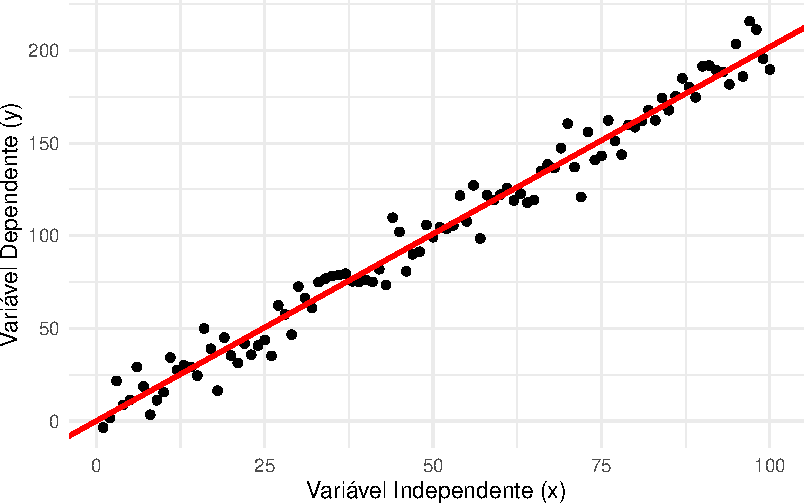
\includegraphics{lista-3_files/figure-pdf/fig-gradiente-1.pdf}

}

\caption{\label{fig-gradiente}Gradiente Descendente para Regressão
Linear}

\end{figure}%

O parâmetro \(\theta\) converge para 2.0197, um valor próximo de 2, que
é a inclinação real da relação entre \(x\) e \(y\). A linha vermelha no
gráfico representa a linha de regressão ajustada, que mostra como o
modelo linear com a inclinação estimada se ajusta aos dados gerados. O
resultado ilustra a eficácia do Gradiente Descendente em encontrar a
inclinação que minimiza o erro quadrático médio entre as previsões e os
valores reais.

\subsection{Algoritmo Perceptron}\label{algoritmo-perceptron}

O Algoritmo Perceptron é um classificador binário que ajusta os pesos
com base nos erros de classificação.

\subsubsection{Principais Conceitos}\label{principais-conceitos}

\begin{itemize}
\tightlist
\item
  \textbf{Classificação Binária}: O Perceptron é capaz de separar duas
  classes linearmente separáveis através de uma função de decisão
  linear.
\item
  \textbf{Aprendizado Supervisionado}: Utiliza rótulos conhecidos para
  aprender a fronteira de decisão, ajustando iterativamente os pesos.
\end{itemize}

\subsubsection{Formulação
Matemática}\label{formulauxe7uxe3o-matemuxe1tica}

O Perceptron ajusta os pesos \(\boldsymbol{w}\) e o viés \(b\) usando a
regra de atualização:

\[
\boldsymbol{w} \leftarrow \boldsymbol{w} + \eta (y_i - \hat{y}_i) \boldsymbol{x}_i
\] onde \(\eta\) é a taxa de aprendizado, \(y_i\) é o rótulo verdadeiro,
\(\hat{y}_i\) é a previsão, e \(\boldsymbol{x}_i\) são as
características de entrada.

\subsubsection{Exemplo}\label{exemplo}

\begin{Shaded}
\begin{Highlighting}[]
\CommentTok{\# Carregar a biblioteca ggplot2}
\FunctionTok{library}\NormalTok{(ggplot2)}

\CommentTok{\# Define uma semente aleatória para garantir que os resultados sejam reprodutíveis}
\FunctionTok{set.seed}\NormalTok{(}\DecValTok{42}\NormalTok{)}

\CommentTok{\# Gera uma matriz 100x2 de números aleatórios normalmente distribuídos}
\NormalTok{x }\OtherTok{\textless{}{-}} \FunctionTok{matrix}\NormalTok{(}\FunctionTok{rnorm}\NormalTok{(}\DecValTok{200}\NormalTok{), }\DecValTok{100}\NormalTok{, }\DecValTok{2}\NormalTok{)}

\CommentTok{\# Cria um vetor com 100 elementos, sendo os primeiros 50 elementos {-}1 e os últimos 50 elementos 1}
\NormalTok{y }\OtherTok{\textless{}{-}} \FunctionTok{c}\NormalTok{(}\FunctionTok{rep}\NormalTok{(}\SpecialCharTok{{-}}\DecValTok{1}\NormalTok{, }\DecValTok{50}\NormalTok{), }\FunctionTok{rep}\NormalTok{(}\DecValTok{1}\NormalTok{, }\DecValTok{50}\NormalTok{))}

\CommentTok{\# Aumenta todos os valores nas duas colunas de \textquotesingle{}x\textquotesingle{} para as entradas onde \textquotesingle{}y\textquotesingle{} é 1}
\NormalTok{x[y }\SpecialCharTok{==} \DecValTok{1}\NormalTok{, ] }\OtherTok{\textless{}{-}}\NormalTok{ x[y }\SpecialCharTok{==} \DecValTok{1}\NormalTok{, ] }\SpecialCharTok{+} \DecValTok{1}

\CommentTok{\# Converte os arrays \textquotesingle{}x\textquotesingle{} e \textquotesingle{}y\textquotesingle{} em um data frame chamado \textquotesingle{}df\textquotesingle{} e transforma \textquotesingle{}y\textquotesingle{} em um fator}
\NormalTok{df }\OtherTok{\textless{}{-}} \FunctionTok{data.frame}\NormalTok{(}\AttributeTok{x1 =}\NormalTok{ x[, }\DecValTok{1}\NormalTok{], }\AttributeTok{x2 =}\NormalTok{ x[, }\DecValTok{2}\NormalTok{], }\AttributeTok{class =} \FunctionTok{as.factor}\NormalTok{(y))}

\CommentTok{\# Inicializa um vetor de pesos com zeros, com um elemento a mais do que o número de colunas em \textquotesingle{}x\textquotesingle{}}
\NormalTok{weights }\OtherTok{\textless{}{-}} \FunctionTok{rep}\NormalTok{(}\DecValTok{0}\NormalTok{, }\FunctionTok{ncol}\NormalTok{(x) }\SpecialCharTok{+} \DecValTok{1}\NormalTok{)}

\CommentTok{\# Define a função Perceptron para ajustar os pesos com base nas entradas \textquotesingle{}x\textquotesingle{}, \textquotesingle{}y\textquotesingle{}, pesos existentes e taxa de aprendizado}
\NormalTok{perceptron }\OtherTok{\textless{}{-}} \ControlFlowTok{function}\NormalTok{(x, y, weights, }\AttributeTok{learning\_rate =} \FloatTok{0.01}\NormalTok{) \{}
  \ControlFlowTok{for}\NormalTok{ (i }\ControlFlowTok{in} \DecValTok{1}\SpecialCharTok{:}\FunctionTok{length}\NormalTok{(y)) \{}
    \CommentTok{\# Verifica se a classificação atual está correta, ajusta os pesos se estiver errada}
    \ControlFlowTok{if}\NormalTok{ (y[i] }\SpecialCharTok{*}\NormalTok{ (}\FunctionTok{crossprod}\NormalTok{(weights, }\FunctionTok{c}\NormalTok{(}\DecValTok{1}\NormalTok{, x[i, ]))) }\SpecialCharTok{\textless{}=} \DecValTok{0}\NormalTok{) \{}
\NormalTok{      weights }\OtherTok{\textless{}{-}}\NormalTok{ weights }\SpecialCharTok{+}\NormalTok{ learning\_rate }\SpecialCharTok{*}\NormalTok{ y[i] }\SpecialCharTok{*} \FunctionTok{c}\NormalTok{(}\DecValTok{1}\NormalTok{, x[i, ])}
\NormalTok{    \}}
\NormalTok{  \}}
  \FunctionTok{return}\NormalTok{(weights)}
\NormalTok{\}}

\CommentTok{\# Treina o modelo Perceptron por 10 épocas, atualizando os pesos a cada iteração}
\ControlFlowTok{for}\NormalTok{ (epoch }\ControlFlowTok{in} \DecValTok{1}\SpecialCharTok{:}\DecValTok{10}\NormalTok{) \{}
\NormalTok{  weights }\OtherTok{\textless{}{-}} \FunctionTok{perceptron}\NormalTok{(x, y, weights)}
\NormalTok{\}}

\CommentTok{\# Calcula a inclinação e a interceptação da linha de decisão baseada nos pesos finais}
\NormalTok{slope }\OtherTok{\textless{}{-}} \SpecialCharTok{{-}}\NormalTok{weights[}\DecValTok{2}\NormalTok{]}\SpecialCharTok{/}\NormalTok{weights[}\DecValTok{3}\NormalTok{]}
\NormalTok{intercept }\OtherTok{\textless{}{-}} \SpecialCharTok{{-}}\NormalTok{weights[}\DecValTok{1}\NormalTok{]}\SpecialCharTok{/}\NormalTok{weights[}\DecValTok{3}\NormalTok{]}
\end{Highlighting}
\end{Shaded}

\begin{Shaded}
\begin{Highlighting}[]
\CommentTok{\# Configura o gráfico ggplot para \textquotesingle{}df\textquotesingle{}, mapeando \textquotesingle{}x1\textquotesingle{} e \textquotesingle{}x2\textquotesingle{} para os eixos x e y, e \textquotesingle{}class\textquotesingle{} para a cor}
\FunctionTok{ggplot}\NormalTok{(df, }\FunctionTok{aes}\NormalTok{(}\AttributeTok{x =}\NormalTok{ x1, }\AttributeTok{y =}\NormalTok{ x2, }\AttributeTok{color =}\NormalTok{ class)) }\SpecialCharTok{+}
  \FunctionTok{geom\_point}\NormalTok{() }\SpecialCharTok{+}  \CommentTok{\# Adiciona pontos ao gráfico para representar as observações}
  \FunctionTok{geom\_abline}\NormalTok{(}\AttributeTok{slope =}\NormalTok{ slope, }\AttributeTok{intercept =}\NormalTok{ intercept, }\AttributeTok{color =} \StringTok{"green"}\NormalTok{, }\AttributeTok{linewidth =} \DecValTok{1}\NormalTok{) }\SpecialCharTok{+}  \CommentTok{\# Adiciona uma linha de decisão}
  \FunctionTok{labs}\NormalTok{(}\AttributeTok{x =} \StringTok{"Feature 1"}\NormalTok{, }\AttributeTok{y =} \StringTok{"Feature 2"}\NormalTok{) }\SpecialCharTok{+}  \CommentTok{\# Define os títulos e rótulos dos eixos}
  \FunctionTok{scale\_color\_manual}\NormalTok{(}\AttributeTok{values =} \FunctionTok{c}\NormalTok{(}\StringTok{"red"}\NormalTok{, }\StringTok{"blue"}\NormalTok{)) }\SpecialCharTok{+}  \CommentTok{\# Define cores manuais para as classes}
  \FunctionTok{theme\_minimal}\NormalTok{()  }\CommentTok{\# Aplica um tema minimalista ao gráfico}
\end{Highlighting}
\end{Shaded}

\begin{figure}[H]

\centering{

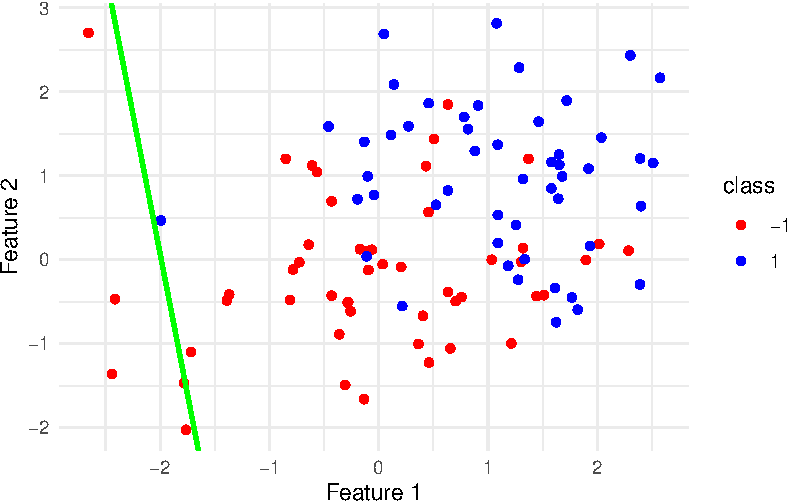
\includegraphics{lista-3_files/figure-pdf/fig-perceptron-1.pdf}

}

\caption{\label{fig-perceptron}Classificação do Perceptron}

\end{figure}%

O Perceptron ajusta uma fronteira de decisão (linha verde) que tenta
separar os pontos de dados em duas classes (vermelho e azul). Os pesos
são ajustados baseados em erros de classificação, e o resultado visual
mostra como a linha foi capaz de separar as duas classes após o
treinamento.

O resultado do algoritmo Perceptron inclui:

\begin{itemize}
\tightlist
\item
  \textbf{Modelo de Classificação Treinado}: O Perceptron é um
  classificador linear binário que aprende a distinguir entre duas
  classes (-1 e 1 nesse caso). O treinamento ajusta os pesos associados
  a cada atributo dos dados (e um peso de viés) de modo que o modelo
  possa corretamente classificar novos exemplos baseado em suas
  características.
\item
  \textbf{Pesos Ajustados}: Ao final do treinamento, os pesos
  representam os parâmetros de um hiperplano que melhor separa as duas
  classes no espaço de características. Esses pesos determinam como as
  entradas (características dos dados) são linearmente combinadas para
  fazer uma previsão de classe.
\item
  \textbf{Fronteira de Decisão}: No espaço bidimensional do exemplo,
  essa fronteira é representada por uma linha reta. A posição e
  orientação dessa linha são diretamente determinadas pelos pesos
  resultantes do treinamento.
\end{itemize}

\subsection{Critério de Fisher}\label{crituxe9rio-de-fisher}

O Critério de Fisher, ou Análise Discriminante Linear (LDA), é uma
técnica que busca maximizar a separação entre diferentes classes
enquanto minimiza a dispersão dentro de cada classe. É usado
primariamente para reduzir a dimensionalidade dos dados antes da
classificação, melhorando assim a eficácia dos modelos de aprendizado de
máquina em ambientes de alta dimensionalidade.

\subsubsection{Principais Conceitos}\label{principais-conceitos-1}

\begin{itemize}
\tightlist
\item
  \textbf{Variância entre as Classes}: Maximiza a distância entre as
  médias das classes.
\item
  \textbf{Variância dentro das Classes}: Minimiza a dispersão dos dados
  dentro de cada classe.
\end{itemize}

\subsubsection{Formulação
Matemática}\label{formulauxe7uxe3o-matemuxe1tica-1}

O vetor de projeção \(\mathbf{w}\) é determinado maximizando a razão:

\[
J(\mathbf{w}) = \frac{\sigma_{\text{entre}}^2}{\sigma_{\text{dentro}}^2}
\] onde \(\sigma_{\text{entre}}^2\) e \(\sigma_{\text{dentro}}^2\)
representam, respectivamente, a variância entre as médias das classes e
a soma das variâncias dentro de cada classe projetada.

\subsubsection{Exemplo}\label{exemplo-1}

\begin{Shaded}
\begin{Highlighting}[]
\CommentTok{\# Filtrar o conjunto de dados iris para excluir a espécie \textquotesingle{}virginica\textquotesingle{}}
\NormalTok{iris\_subset }\OtherTok{\textless{}{-}} \FunctionTok{droplevels}\NormalTok{(iris[iris}\SpecialCharTok{$}\NormalTok{Species }\SpecialCharTok{!=} \StringTok{"virginica"}\NormalTok{, ])}

\CommentTok{\# Ajustar o modelo LDA ao subconjunto de dados}
\NormalTok{model }\OtherTok{\textless{}{-}} \FunctionTok{lda}\NormalTok{(Species }\SpecialCharTok{\textasciitilde{}}\NormalTok{ ., }\AttributeTok{data =}\NormalTok{ iris\_subset)}

\CommentTok{\# Obter as projeções LDA usando predict}
\NormalTok{projection }\OtherTok{\textless{}{-}} \FunctionTok{predict}\NormalTok{(model)}\SpecialCharTok{$}\NormalTok{x  }\CommentTok{\# Isto obtém os valores discriminantes diretamente}

\CommentTok{\# Converter projeções e espécies em um dataframe para uso no ggplot}
\NormalTok{plot\_data }\OtherTok{\textless{}{-}} \FunctionTok{data.frame}\NormalTok{(}\AttributeTok{Index =} \DecValTok{1}\SpecialCharTok{:}\FunctionTok{nrow}\NormalTok{(projection), }\AttributeTok{Projection =}\NormalTok{ projection[,}\DecValTok{1}\NormalTok{], }\AttributeTok{Species =}\NormalTok{ iris\_subset}\SpecialCharTok{$}\NormalTok{Species)}
\end{Highlighting}
\end{Shaded}

\begin{Shaded}
\begin{Highlighting}[]
\CommentTok{\# Criar o gráfico usando ggplot}
\FunctionTok{ggplot}\NormalTok{(plot\_data, }\FunctionTok{aes}\NormalTok{(}\AttributeTok{x =}\NormalTok{ Projection, }\AttributeTok{y =}\NormalTok{ Index, }\AttributeTok{color =}\NormalTok{ Species)) }\SpecialCharTok{+}
  \FunctionTok{geom\_point}\NormalTok{(}\AttributeTok{alpha =} \FloatTok{0.6}\NormalTok{) }\SpecialCharTok{+}  \CommentTok{\# Use alpha para ajustar a transparência, se necessário}
  \FunctionTok{labs}\NormalTok{(}\AttributeTok{x =} \StringTok{"Projection"}\NormalTok{, }\AttributeTok{y =} \StringTok{"Index"}\NormalTok{) }\SpecialCharTok{+}
  \FunctionTok{scale\_color\_brewer}\NormalTok{(}\AttributeTok{palette =} \StringTok{"Set1"}\NormalTok{, }\AttributeTok{name =} \StringTok{"Species"}\NormalTok{) }\SpecialCharTok{+}
  \FunctionTok{theme\_minimal}\NormalTok{()}
\end{Highlighting}
\end{Shaded}

\begin{figure}[H]

\centering{

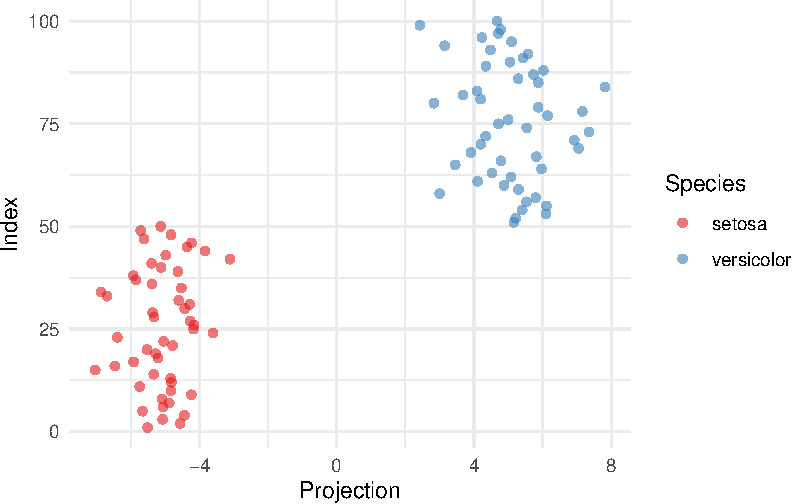
\includegraphics{lista-3_files/figure-pdf/fig-lda-1.pdf}

}

\caption{\label{fig-lda}Projeção LDA com Critério de Fisher}

\end{figure}%

O gráfico mostra a eficácia da projeção LDA em separar duas espécies de
íris, utilizando o Critério de Fisher para maximizar a distância entre
as classes.

\subsection{Critério de Mínimos
Quadrados}\label{crituxe9rio-de-muxednimos-quadrados}

O Critério de Mínimos Quadrados é usado para estimar os coeficientes de
um modelo de regressão. O objetivo é minimizar a soma dos quadrados das
diferenças entre os valores observados e os valores estimados pelo
modelo, garantindo assim a melhor adequação possível dos dados ao modelo
encontrado.

\subsubsection{Principais Conceitos}\label{principais-conceitos-2}

\begin{itemize}
\tightlist
\item
  \textbf{Erro Quadrático}: Mede a diferença ao quadrado entre os
  valores observados e os preditos pelo modelo.
\item
  \textbf{Ajuste de Modelo}: O critério busca parâmetros que reduzam ao
  mínimo o erro quadrático total, refletindo a melhor previsão possível
  dada a variabilidade dos dados.
\end{itemize}

\subsubsection{Formulação
Matemática}\label{formulauxe7uxe3o-matemuxe1tica-2}

A estimativa dos coeficientes do modelo de regressão é realizada através
da solução da equação:

\[
\beta = (\mathbf{X}^\top\mathbf{X})^{-1} \mathbf{X}^\top\mathbf{y}
\] onde \(\mathbf{X}\) representa a matriz de dados (com uma coluna
adicional de uns para o intercepto), \(\beta\) são os coeficientes a
serem estimados, e \(\mathbf{y}\) é o vetor de variáveis dependentes.

\subsubsection{Exemplo}\label{exemplo-2}

\begin{Shaded}
\begin{Highlighting}[]
\CommentTok{\# Gerar 100 números aleatórios normalmente distribuídos como variável independente \textquotesingle{}x\textquotesingle{}}
\NormalTok{x }\OtherTok{\textless{}{-}} \FunctionTok{rnorm}\NormalTok{(}\DecValTok{100}\NormalTok{)}

\CommentTok{\# Criar a variável dependente \textquotesingle{}y\textquotesingle{} como uma função linear de \textquotesingle{}x\textquotesingle{} mais ruído gaussiano}
\NormalTok{y }\OtherTok{\textless{}{-}} \DecValTok{2} \SpecialCharTok{*}\NormalTok{ x }\SpecialCharTok{+} \FunctionTok{rnorm}\NormalTok{(}\DecValTok{100}\NormalTok{)}

\CommentTok{\# Criar um data frame a partir de x e y}
\NormalTok{data }\OtherTok{\textless{}{-}} \FunctionTok{data.frame}\NormalTok{(x, y)}

\CommentTok{\# Ajustar um modelo de regressão linear onde \textquotesingle{}y\textquotesingle{} é predito por \textquotesingle{}x\textquotesingle{}}
\NormalTok{model }\OtherTok{\textless{}{-}} \FunctionTok{lm}\NormalTok{(y }\SpecialCharTok{\textasciitilde{}}\NormalTok{ x, }\AttributeTok{data =}\NormalTok{ data)}

\CommentTok{\# Criar um gráfico de dispersão usando ggplot}
\NormalTok{MQ }\OtherTok{\textless{}{-}} \FunctionTok{ggplot}\NormalTok{(data, }\FunctionTok{aes}\NormalTok{(}\AttributeTok{x =}\NormalTok{ x, }\AttributeTok{y =}\NormalTok{ y)) }\SpecialCharTok{+}
  \FunctionTok{geom\_point}\NormalTok{() }\SpecialCharTok{+}  \CommentTok{\# Adicionar pontos ao gráfico}
  \FunctionTok{geom\_smooth}\NormalTok{(}\AttributeTok{method =} \StringTok{"lm"}\NormalTok{, }\AttributeTok{se =} \ConstantTok{FALSE}\NormalTok{, }\AttributeTok{color =} \StringTok{"red"}\NormalTok{, }\AttributeTok{size =} \DecValTok{1}\NormalTok{) }\SpecialCharTok{+}  \CommentTok{\# Adicionar linha de regressão}
  \FunctionTok{labs}\NormalTok{(}\AttributeTok{title =} \StringTok{"Regressão Linear com Mínimos Quadrados"}\NormalTok{, }\AttributeTok{x =} \StringTok{"Variável Independente (x)"}\NormalTok{, }\AttributeTok{y =} \StringTok{"Variável Dependente (y)"}\NormalTok{) }\SpecialCharTok{+}
  \FunctionTok{theme\_minimal}\NormalTok{()  }\CommentTok{\# Utilizar um tema minimalista para o gráfico}

\CommentTok{\# Exibir o gráfico}
\FunctionTok{print}\NormalTok{(MQ)}
\end{Highlighting}
\end{Shaded}

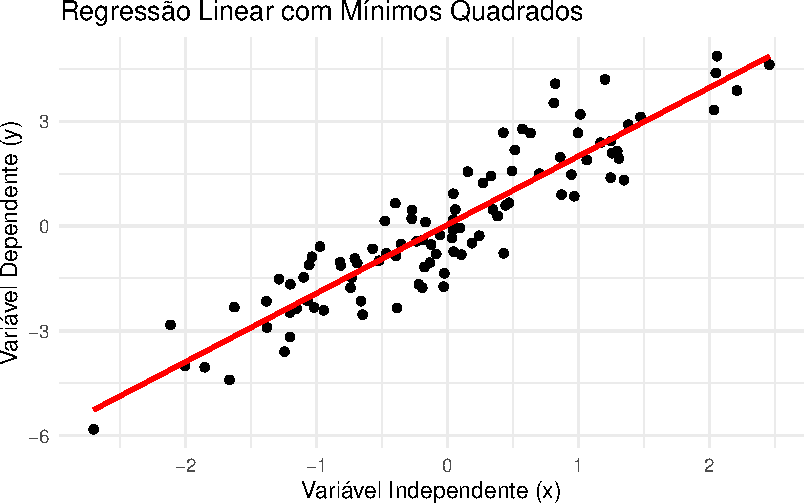
\includegraphics{lista-3_files/figure-pdf/unnamed-chunk-8-1.pdf}

A linha vermelha mostra a melhor ajuste linear, minimizando as
diferenças quadradas entre os valores observados e preditos,
demonstrando a precisão do modelo na estimativa da relação entre as
variáveis.

\newpage{}

\section{Questão 7}\label{questuxe3o-7}

Estudar e apresentar um exemplo utilizando as notas sobre Perceptron no
R descritas em \url{https://rpubs.com/FaiHas/197581}.

\begin{center}\rule{0.5\linewidth}{0.5pt}\end{center}

O autor apresenta o algoritmo de Frank Rosenblatt para classificação. O
exemplo apresentado considera uma base de dados contendo uma lista de
pesos e rótulos indicando a espécie de íris do banco de dados
\texttt{datasets::iris}. O perceptron recebe a base de dados e
``aprende'' a identificar as classes corretamente com base nas
características da observação.

A base de dados \texttt{iris} original é composta por 150 observações de
4 variáveis (comprimento e largura da sépala e pétala) e 1 variável de
classe (espécie da íris). O autor utiliza um subconjunto de 100
observações aleatórias da base de dados e cria um vetor de rótulos
binários para as espécies ``setosa'' e ``versicolor''.

~

\begin{Shaded}
\begin{Highlighting}[]
\NormalTok{irissubdf }\OtherTok{\textless{}{-}}\NormalTok{ iris[}\DecValTok{1}\SpecialCharTok{:}\DecValTok{100}\NormalTok{, }\FunctionTok{c}\NormalTok{(}\DecValTok{1}\NormalTok{, }\DecValTok{3}\NormalTok{, }\DecValTok{5}\NormalTok{)]}
\FunctionTok{names}\NormalTok{(irissubdf) }\OtherTok{\textless{}{-}} \FunctionTok{c}\NormalTok{(}\StringTok{"sepal"}\NormalTok{, }\StringTok{"petal"}\NormalTok{, }\StringTok{"species"}\NormalTok{)}
\FunctionTok{head}\NormalTok{(irissubdf) }\SpecialCharTok{\%\textgreater{}\%}
\NormalTok{  knitr}\SpecialCharTok{::}\FunctionTok{kable}\NormalTok{()}
\end{Highlighting}
\end{Shaded}

\begin{longtable}[]{@{}rrl@{}}

\caption{\label{tbl-subsetiris}Subconjunto de Dados Iris}

\tabularnewline

\toprule\noalign{}
sepal & petal & species \\
\midrule\noalign{}
\endhead
\bottomrule\noalign{}
\endlastfoot
5.1 & 1.4 & setosa \\
4.9 & 1.4 & setosa \\
4.7 & 1.3 & setosa \\
4.6 & 1.5 & setosa \\
5.0 & 1.4 & setosa \\
5.4 & 1.7 & setosa \\

\end{longtable}

~

O subconjunto de dados é exibido na Figura~\ref{fig-plotsubsetiris} a
seguir.

~

\begin{Shaded}
\begin{Highlighting}[]
\FunctionTok{ggplot}\NormalTok{(irissubdf, }\FunctionTok{aes}\NormalTok{(}\AttributeTok{x =}\NormalTok{ sepal, }\AttributeTok{y =}\NormalTok{ petal,}
                      \AttributeTok{colour=}\NormalTok{species, }\AttributeTok{shape=}\NormalTok{ species)) }\SpecialCharTok{+} 
        \FunctionTok{geom\_point}\NormalTok{(}\AttributeTok{size =} \DecValTok{3}\NormalTok{) }\SpecialCharTok{+}
        \FunctionTok{labs}\NormalTok{(}\AttributeTok{x =} \StringTok{"Comp. Sépala"}\NormalTok{, }\AttributeTok{y =} \StringTok{"Comp. Pétala"}\NormalTok{)}\SpecialCharTok{+}
  \FunctionTok{theme\_bw}\NormalTok{()}\SpecialCharTok{+}
  \FunctionTok{theme}\NormalTok{(}\AttributeTok{legend.title =} \FunctionTok{element\_blank}\NormalTok{())}
\end{Highlighting}
\end{Shaded}

\begin{figure}[H]

\centering{

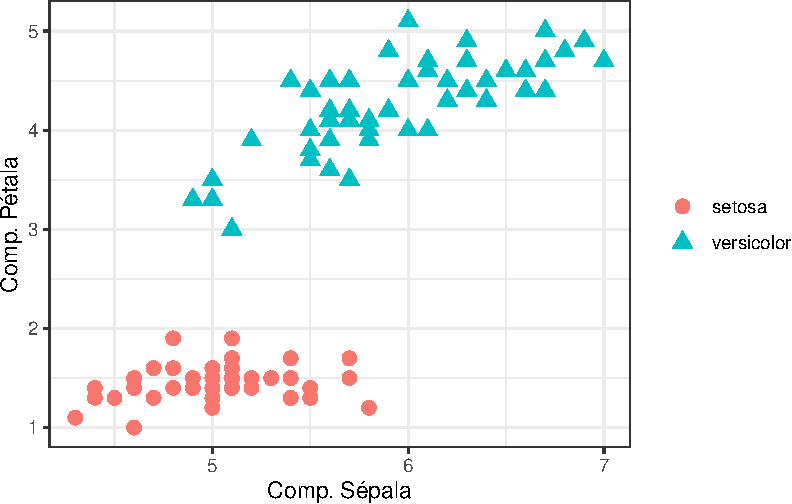
\includegraphics{lista-3_files/figure-pdf/fig-plotsubsetiris-1.pdf}

}

\caption{\label{fig-plotsubsetiris}Espécies em função de comprimento de
sépala e pétala}

\end{figure}%

~

Em seguida, o autor adiciona uma quarta variável ao subconjunto de dados
representando o rótulo. Se a espécie for ``setosa'', o rótulo é 1; caso
contrário, o rótulo é -1. Em seguida, as características são atribuídas
ao objeto \texttt{x} e os rótulos ao objeto \texttt{y}.

~

\begin{Shaded}
\begin{Highlighting}[]
\NormalTok{irissubdf }\OtherTok{\textless{}{-}}\NormalTok{ irissubdf }\SpecialCharTok{\%\textgreater{}\%}
  \FunctionTok{mutate}\NormalTok{(}\AttributeTok{label =} \FunctionTok{case\_when}\NormalTok{(}
\NormalTok{    species }\SpecialCharTok{==} \StringTok{"setosa"} \SpecialCharTok{\textasciitilde{}} \DecValTok{1}\NormalTok{,}
\NormalTok{    species }\SpecialCharTok{==} \StringTok{"versicolor"} \SpecialCharTok{\textasciitilde{}} \SpecialCharTok{{-}}\DecValTok{1}
\NormalTok{  ))}

\NormalTok{x }\OtherTok{\textless{}{-}}\NormalTok{ irissubdf }\SpecialCharTok{\%\textgreater{}\%}\NormalTok{ dplyr}\SpecialCharTok{::}\FunctionTok{select}\NormalTok{(sepal, petal)}
\NormalTok{y }\OtherTok{\textless{}{-}}\NormalTok{ irissubdf }\SpecialCharTok{\%\textgreater{}\%}\NormalTok{ dplyr}\SpecialCharTok{::}\FunctionTok{select}\NormalTok{(label) }\SpecialCharTok{\%\textgreater{}\%} \FunctionTok{pull}\NormalTok{()}
\end{Highlighting}
\end{Shaded}

~

Finalmente, o algoritmo perceptron é implementado na mesma forma que foi
apresentado nas notas de aula. A função que o executa recebe quatro
argumentos: dados, rótulos, taxa de aprendizagem e número de iterações.

A função é inicializada com um vetor de pesos
\(\boldsymbol{w} = (w_1 = 0, w_2 = 0, b = 0)\) e um vetor nulo de erros
do mesmo tamanho que o número de iterações. O algoritmo percorre o
conjunto de dados e ajusta os pesos de acordo com a regra de atualização
do perceptron em dois laços:

\begin{itemize}
\tightlist
\item
  o primeiro laço percorre o número de iterações;
\item
  o segundo laço percorre o número de observações em cada iteração.
\end{itemize}

No algoritmo, \(z = \boldsymbol{w}^\top\boldsymbol{x} + b\) é a previsão
da observação com os pesos correntes, porém é feito elemento a elemento.
Se \(z < 0\), a previsão é -1; caso contrário, a previsão é 1. Os pesos
são atualizados da seguinte forma para cada observação \(i\):

\[
  \boldsymbol{w}^{(t)} \leftarrow \boldsymbol{w}^{(t-1)} + \eta (y_i - \hat{y}_i) \begin{bmatrix} 1 \\ \boldsymbol{x}_i \end{bmatrix}
\]

\noindent em que \(\eta\) é a taxa de aprendizagem. Nota-se que o peso
\emph{não} é atualizado se a classificação for correta. O vetor

Depois de percorrer a base de dados completa em cada iteração, o erro é
atualizado se a classificação for incorreta. O vetor final de erros da
função indica quantas classificações erradas foram feitas em cada
iteração.

Finalmente, uma pequena alteração foi feita na função para que seja
retornada uma lista com dois elementos: o vetor de pesos e o vetor de
erros.

~

\begin{Shaded}
\begin{Highlighting}[]
\NormalTok{perceptron }\OtherTok{\textless{}{-}} \ControlFlowTok{function}\NormalTok{(x, y, eta, niter) \{}
        
        \CommentTok{\# initialize weight vector}
\NormalTok{        weight }\OtherTok{\textless{}{-}} \FunctionTok{rep}\NormalTok{(}\DecValTok{0}\NormalTok{, }\FunctionTok{dim}\NormalTok{(x)[}\DecValTok{2}\NormalTok{] }\SpecialCharTok{+} \DecValTok{1}\NormalTok{)}
\NormalTok{        errors }\OtherTok{\textless{}{-}} \FunctionTok{rep}\NormalTok{(}\DecValTok{0}\NormalTok{, niter)}
        
        
        \CommentTok{\# loop over number of epochs niter}
        \ControlFlowTok{for}\NormalTok{ (jj }\ControlFlowTok{in} \DecValTok{1}\SpecialCharTok{:}\NormalTok{niter) \{}
                
                \CommentTok{\# loop through training data set}
                \ControlFlowTok{for}\NormalTok{ (ii }\ControlFlowTok{in} \DecValTok{1}\SpecialCharTok{:}\FunctionTok{length}\NormalTok{(y)) \{}
                        
                        \CommentTok{\# Predict binary label using Heaviside activation }
                        \CommentTok{\# function}
\NormalTok{                        z }\OtherTok{\textless{}{-}} \FunctionTok{sum}\NormalTok{(weight[}\DecValTok{2}\SpecialCharTok{:}\FunctionTok{length}\NormalTok{(weight)] }\SpecialCharTok{*} 
                                         \FunctionTok{as.numeric}\NormalTok{(x[ii, ])) }\SpecialCharTok{+}\NormalTok{ weight[}\DecValTok{1}\NormalTok{]}
                        \ControlFlowTok{if}\NormalTok{(z }\SpecialCharTok{\textless{}} \DecValTok{0}\NormalTok{) \{}
\NormalTok{                                ypred }\OtherTok{\textless{}{-}} \SpecialCharTok{{-}}\DecValTok{1}
\NormalTok{                        \} }\ControlFlowTok{else}\NormalTok{ \{}
\NormalTok{                                ypred }\OtherTok{\textless{}{-}} \DecValTok{1}
\NormalTok{                        \}}
                        
                        \CommentTok{\# Change weight {-} the formula doesn\textquotesingle{}t do anything }
                        \CommentTok{\# if the predicted value is correct}
\NormalTok{                        weightdiff }\OtherTok{\textless{}{-}}\NormalTok{ eta }\SpecialCharTok{*}\NormalTok{ (y[ii] }\SpecialCharTok{{-}}\NormalTok{ ypred) }\SpecialCharTok{*} 
                                \FunctionTok{c}\NormalTok{(}\DecValTok{1}\NormalTok{, }\FunctionTok{as.numeric}\NormalTok{(x[ii, ]))}
\NormalTok{                        weight }\OtherTok{\textless{}{-}}\NormalTok{ weight }\SpecialCharTok{+}\NormalTok{ weightdiff}
                        
                        \CommentTok{\# Update error function}
                        \ControlFlowTok{if}\NormalTok{ ((y[ii] }\SpecialCharTok{{-}}\NormalTok{ ypred) }\SpecialCharTok{!=} \FloatTok{0.0}\NormalTok{) \{}
\NormalTok{                                errors[jj] }\OtherTok{\textless{}{-}}\NormalTok{ errors[jj] }\SpecialCharTok{+} \DecValTok{1}
\NormalTok{                        \}}
                        
\NormalTok{                \}}
\NormalTok{        \}}
        
        \CommentTok{\# weight to decide between the two species }
        \FunctionTok{return}\NormalTok{(}\FunctionTok{list}\NormalTok{(}
          \AttributeTok{w =}\NormalTok{ weight,}
          \AttributeTok{erros =}\NormalTok{ errors)}
\NormalTok{          )}
\NormalTok{\}}
\end{Highlighting}
\end{Shaded}

~

Com o subconjunto escolhido pelo autor, obtemos o vetor de pesos

\begin{Shaded}
\begin{Highlighting}[]
\NormalTok{pesos\_iris}\OtherTok{\textless{}{-}} \FunctionTok{perceptron}\NormalTok{(x, y, }\DecValTok{1}\NormalTok{, }\DecValTok{10}\NormalTok{)}
\end{Highlighting}
\end{Shaded}

\begin{align}
  \boldsymbol{w} = \begin{bmatrix} 4 \\ 7 \end{bmatrix} \quad b = -18.4
 \end{align}

\noindent e a quantidade de erros por iterações, apresentada na
Figura~\ref{fig-errosperceptron} a seguir, um pouco diferente do que o
autor exibe.

~

\begin{Shaded}
\begin{Highlighting}[]
\FunctionTok{ggplot}\NormalTok{(}\AttributeTok{data =} \FunctionTok{as\_tibble}\NormalTok{(pesos\_iris}\SpecialCharTok{$}\NormalTok{erros), }\FunctionTok{aes}\NormalTok{(}\AttributeTok{x =} \DecValTok{1}\SpecialCharTok{:}\FunctionTok{length}\NormalTok{(pesos\_iris}\SpecialCharTok{$}\NormalTok{erros), }\AttributeTok{y =}\NormalTok{ pesos\_iris}\SpecialCharTok{$}\NormalTok{erros)) }\SpecialCharTok{+}
  \FunctionTok{geom\_line}\NormalTok{(}\AttributeTok{color =} \StringTok{"red"}\NormalTok{) }\SpecialCharTok{+}
  \FunctionTok{labs}\NormalTok{(}\AttributeTok{x =} \StringTok{"Iterações"}\NormalTok{, }\AttributeTok{y =} \StringTok{"Erros"}\NormalTok{) }\SpecialCharTok{+}
  \FunctionTok{theme\_bw}\NormalTok{() }\SpecialCharTok{+}
  \FunctionTok{theme}\NormalTok{(}
    \AttributeTok{panel.grid.major.x =} \FunctionTok{element\_blank}\NormalTok{(), }\CommentTok{\# Remove major x grids}
    \AttributeTok{panel.grid.minor.x =} \FunctionTok{element\_blank}\NormalTok{(), }\CommentTok{\# Remove minor x grids}
    \AttributeTok{panel.grid.minor.y =} \FunctionTok{element\_blank}\NormalTok{()  }\CommentTok{\# Remove minor y grids}
\NormalTok{  )}
\end{Highlighting}
\end{Shaded}

\begin{figure}[H]

\centering{

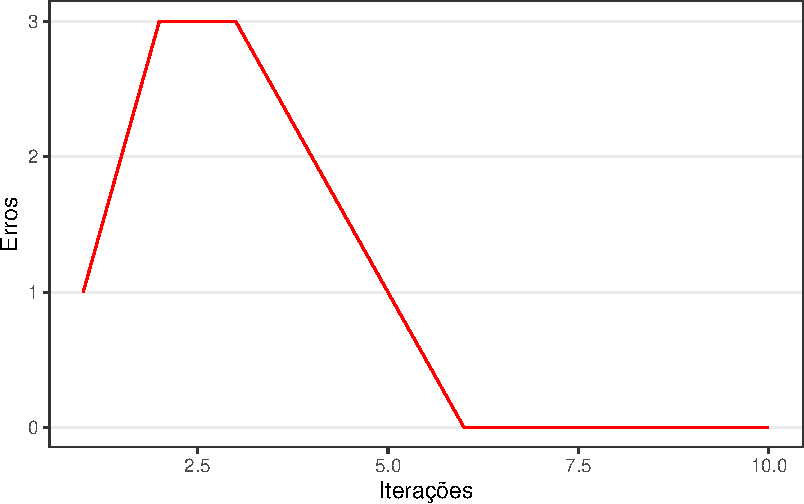
\includegraphics{lista-3_files/figure-pdf/fig-errosperceptron-1.pdf}

}

\caption{\label{fig-errosperceptron}Erros por Iterações do algoritmo
Perceptron}

\end{figure}%

~

O autor finalmente tece comentários sobre classificação multiclasse
usando o perceptron. Trata-se de um algoritmo com baixa capacidade de
representação, sendo adequado apenas para problemas de classificação
binária, portanto seria necessário tanto mais características das
observações quanto procedimentos de classificação do tipo Classe 1
\emph{versus} Demais.

Algo que se é necessário destacar também é que, enquanto o erro de
classificação convergiu para zero no exemplo apresentado, isso não é
garantido para todos os problemas. Com as três espécies, conforme a
Figura~\ref{fig-iris3species} a seguir, duas não são linearmente
separáveis entre si, de modo que o erro converge para um valor superior
a zero para esta configuração do algoritmo.

\begin{Shaded}
\begin{Highlighting}[]
\NormalTok{irisdata }\OtherTok{\textless{}{-}}\NormalTok{ iris[, }\FunctionTok{c}\NormalTok{(}\DecValTok{1}\NormalTok{, }\DecValTok{3}\NormalTok{, }\DecValTok{5}\NormalTok{)]}
\FunctionTok{names}\NormalTok{(irisdata) }\OtherTok{\textless{}{-}} \FunctionTok{c}\NormalTok{(}\StringTok{"sepal"}\NormalTok{, }\StringTok{"petal"}\NormalTok{, }\StringTok{"species"}\NormalTok{)}

\FunctionTok{ggplot}\NormalTok{(irisdata, }\FunctionTok{aes}\NormalTok{(}\AttributeTok{x =}\NormalTok{ sepal, }\AttributeTok{y =}\NormalTok{ petal,}
                      \AttributeTok{colour=}\NormalTok{species, }\AttributeTok{shape=}\NormalTok{ species)) }\SpecialCharTok{+} 
        \FunctionTok{geom\_point}\NormalTok{(}\AttributeTok{size =} \DecValTok{3}\NormalTok{) }\SpecialCharTok{+}
        \FunctionTok{labs}\NormalTok{(}\AttributeTok{x =} \StringTok{"Comp. Sépala"}\NormalTok{, }\AttributeTok{y =} \StringTok{"Comp. Pétala"}\NormalTok{)}\SpecialCharTok{+}
  \FunctionTok{theme\_bw}\NormalTok{()}\SpecialCharTok{+}
  \FunctionTok{theme}\NormalTok{(}\AttributeTok{legend.title =} \FunctionTok{element\_blank}\NormalTok{())}
\end{Highlighting}
\end{Shaded}

\begin{figure}[H]

\centering{

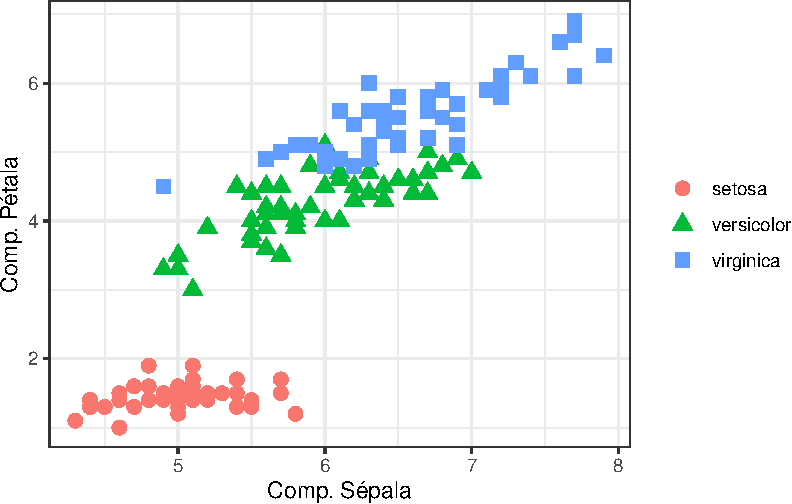
\includegraphics{lista-3_files/figure-pdf/fig-iris3species-1.pdf}

}

\caption{\label{fig-iris3species}Espécies em função de comprimento de
sépala e pétala usando a base iris completa}

\end{figure}%

\newpage{}

\section{Questão 8}\label{questuxe3o-8}

\begin{enumerate}
\def\labelenumi{\alph{enumi})}
\tightlist
\item
  Estudar e apresentar a função perceptron do pacote \texttt{mlpack} do
  R.
\item
  Verificar se existe material adicional (instruções em sites, pacotes,
  artigos) sobre classificação utilizando o algoritmo perceptron no R e
  apresentar exemplos.
\end{enumerate}

\begin{center}\rule{0.5\linewidth}{0.5pt}\end{center}

\subsection{item a)}\label{item-a}

De acordo com a documentação da função
\texttt{mlpack::perceptron()}\footnote{\url{https://www.mlpack.org/doc/mlpack-git/r_documentation.html\#perceptron}},

\emph{``Este programa implementa um perceptron, que é uma rede neural de
nível único. O perceptron faz suas previsões com base em uma função
preditora linear que combina um conjunto de pesos com o vetor de
características. A regra de aprendizado do perceptron é capaz de
convergir, dadas iterações suficientes (especificadas usando o parâmetro
max\_iterations), se os dados fornecidos forem linearmente separáveis. O
perceptron é parametrizado por uma matriz de vetores de peso que denotam
os pesos numéricos da rede neural.}

\emph{Este programa permite carregar um perceptron a partir de um modelo
(via o parâmetro input\_model) ou treinar um perceptron com dados de
treinamento (via o parâmetro training), ou ambas as coisas ao mesmo
tempo. Além disso, este programa permite a classificação em um conjunto
de dados de teste (via o parâmetro test) e os resultados da
classificação no conjunto de teste podem ser salvos com o parâmetro de
saída predictions. O modelo de perceptron pode ser salvo com o parâmetro
de saída output\_model.''}

São 7 os possíveis argumentos de entrada:

\begin{itemize}
\tightlist
\item
  \textbf{check\_input\_matrices}

  \begin{itemize}
  \tightlist
  \item
    \emph{tipo}: lógico
  \item
    \emph{descrição}: Se especificado, a matriz de entrada é verificada
    para valores NaN e inf; uma exceção é lançada se algum for
    encontrado.
  \item
    \emph{padrão}: FALSE
  \end{itemize}
\item
  \textbf{input\_model}

  \begin{itemize}
  \tightlist
  \item
    \emph{tipo}: PerceptronModel
  \item
    \emph{descrição}: Modelo de perceptron de entrada.
  \item
    \emph{padrão}: NA
  \end{itemize}
\item
  \textbf{labels}

  \begin{itemize}
  \tightlist
  \item
    \emph{tipo}: vetor de inteiros
  \item
    \emph{descrição}: Uma matriz contendo os rótulos para o conjunto de
    treinamento.
  \item
    \emph{padrão}: matrix(integer(), 0, 0)
  \end{itemize}
\item
  \textbf{max\_iterations}

  \begin{itemize}
  \tightlist
  \item
    \emph{tipo}: inteiro
  \item
    \emph{descrição}: O número máximo de iterações que o perceptron deve
    executar.
  \item
    \emph{padrão}: 1000
  \end{itemize}
\item
  \textbf{test}

  \begin{itemize}
  \tightlist
  \item
    \emph{tipo}: matriz numérica
  \item
    \emph{descrição}: Uma matriz contendo o conjunto de teste.
  \item
    \emph{padrão}: matrix(numeric(), 0, 0)
  \end{itemize}
\item
  \textbf{training}

  \begin{itemize}
  \tightlist
  \item
    \emph{tipo}: matriz numérica
  \item
    \emph{descrição}: Uma matriz contendo o conjunto de treinamento.
  \item
    \emph{padrão}: matrix(numeric(), 0, 0)
  \end{itemize}
\item
  \textbf{verbose}

  \begin{itemize}
  \tightlist
  \item
    \emph{tipo}: lógico
  \item
    \emph{descrição}: Exibir mensagens informativas e a lista completa
    de parâmetros e temporizadores no final da execução.
  \item
    \emph{padrão}: FALSE
  \end{itemize}
\end{itemize}

~

Os resultados são apresentados em uma lista com os seguintes elementos:

\begin{itemize}
\tightlist
\item
  \textbf{output}

  \begin{itemize}
  \tightlist
  \item
    \emph{tipo}: vetor de inteiros
  \item
    \emph{descrição}: A matriz na qual os rótulos previstos para o
    conjunto de teste serão escritos.
  \end{itemize}
\item
  \textbf{output\_model}

  \begin{itemize}
  \tightlist
  \item
    \emph{tipo}: PerceptronModel
  \item
    \emph{descrição}: Saída para o modelo de perceptron treinado.
  \end{itemize}
\item
  \textbf{predictions}

  \begin{itemize}
  \tightlist
  \item
    \emph{tipo}: vetor de inteiros
  \item
    \emph{descrição}: A matriz na qual os rótulos previstos para o
    conjunto de teste serão escritos.
  \end{itemize}
\end{itemize}

~

\subsection{item b)}\label{item-b}

Enquanto o próprio
\href{https://www.mlpack.org/doc/mlpack-git/r_documentation.html\#perceptron}{mlpack.org}
já traz a documentaçào da função, que é a mesma do CRAN, os próprios
autores têm artigos publicados sobre a elaboração do pacote e seu
desempenho (Edel, Soni, e Curtin 2014; Curtin e Edel 2017).

No entanto, outros materiais, inclusive videos do YouTube, não foram
identificados. Em vez disso, os resultados apresentam tutoriais e teoria
acerca do \emph{multilayer perceptron} --- que é a própria Deep
Learning.

\newpage{}

\section{Questão 9 - Critério de
Fisher}\label{questuxe3o-9---crituxe9rio-de-fisher}

A Análise Discriminante Linear (\emph{Linear Discriminant Analysis} --
LDA) pode ser considerada uma extensão do critério de Fisher para
reconhecimento de padrões, sendo esse um método estatístico que busca
encontrar uma combinação linear dos recursos que melhor discrimina entre
duas ou mais classes.

A utilização dessa técnica no \texttt{R} tem suas vantagens pela
facilidade com a qual pode ser implementada e a versatilidade ao se
integrar com outras funções estatísticas do R, mas pode acabar sofrendo
com conjuntos de dados muito grandes ou necessidades computacionais
muito altas.

\subsection{Exemplo}\label{exemplo-3}

A seguir temos um exemplo da implementação de LDA no banco de dados
Iris, composto classificações de 3 espécies de flores e medidas em
centímetros das variáveis comprimento e largura da sépala e comprimento
e largura da pétala.

\begin{Shaded}
\begin{Highlighting}[]
\FunctionTok{data}\NormalTok{(iris)}
\NormalTok{dados }\OtherTok{\textless{}{-}}\NormalTok{ iris}

\NormalTok{modelo\_discriminante }\OtherTok{\textless{}{-}} \FunctionTok{lda}\NormalTok{( Species }\SpecialCharTok{\textasciitilde{}}\NormalTok{ Sepal.Length }\SpecialCharTok{+}\NormalTok{Sepal.Width}\SpecialCharTok{+}\NormalTok{ Petal.Length }\SpecialCharTok{+}\NormalTok{ Petal.Width, }\AttributeTok{data =}\NormalTok{ dados )}

\NormalTok{data.predic }\OtherTok{\textless{}{-}}\FunctionTok{predict}\NormalTok{(modelo\_discriminante,}\AttributeTok{newdata =}\NormalTok{ dados[,}\DecValTok{1}\SpecialCharTok{:}\DecValTok{4}\NormalTok{])}\SpecialCharTok{$}\NormalTok{class}
\end{Highlighting}
\end{Shaded}

A Tabela~\ref{tbl-lda} a seguir apresenta a quantidade de classificações
corretas e a quantidade de classificações erradas a partir do nosso
modelo ajustado.

\begin{Shaded}
\begin{Highlighting}[]
\FunctionTok{table}\NormalTok{(data.predic, dados[,}\DecValTok{5}\NormalTok{]) }\SpecialCharTok{\%\textgreater{}\%}
\NormalTok{  knitr}\SpecialCharTok{::}\FunctionTok{kable}\NormalTok{()}
\end{Highlighting}
\end{Shaded}

\begin{longtable}[]{@{}lrrr@{}}

\caption{\label{tbl-lda}Tabela de Classificações Corretas e Incorretas
do LDA}

\tabularnewline

\toprule\noalign{}
& setosa & versicolor & virginica \\
\midrule\noalign{}
\endhead
\bottomrule\noalign{}
\endlastfoot
setosa & 50 & 0 & 0 \\
versicolor & 0 & 48 & 1 \\
virginica & 0 & 2 & 49 \\

\end{longtable}

~

A Figura~\ref{fig-ldairis} a seguir nos mostra como, a partir dos
Discriminates lineares estimados do nosso modelo LDA, as divisões de
classes foram feitas. O eixo LDA1 representa a direção da máxima
separação entre as classes, enquanto o eixo LDA2 representa a direção da
segunda maior separação.

O diagrama de dispersão demonstra uma clara separação entre as três
classes de flores de íris. As flores setosa estão agrupadas no canto
superior direito do gráfico, as flores versicolor e flores virginica
estão agrupadas no canto inferior esquerdo distribuídas entre os dois
aglomerados. As flores setosa são as mais bem agrupadas, indicando menor
variabilidade dentro dessa classe. As flores versicolor e virgínica
estão mais espalhadas, sugerindo maior variabilidade dentro dessas duas
classes

O ponto marcado por X em cada classe de plantas indica a sua média
geral. Assim,

\begin{itemize}
\tightlist
\item
  \emph{Setosa}: indica que a sua média tem um valor LDA1 positivo e um
  valor LDA2 negativo tendo a maior diferença em relação à média geral
  entre as três classes.
\item
  \emph{Virginica}: indica que a sua média tem um valor LDA1 negativo e
  um valor LDA2 positivo tendo a segunda maior diferença em relação à
  média geral entre as três classes.
\item
  \emph{Versicolor}: indica que a sua média tem um valor negativo tanto
  para LD1 quanto para LD2, mas perto de 0 tendo a menor diferença em
  relaçao a média geral.
\end{itemize}

~

\begin{Shaded}
\begin{Highlighting}[]
\CommentTok{\# Obter as predições do modelo LDA}
\NormalTok{lda\_pred }\OtherTok{\textless{}{-}} \FunctionTok{predict}\NormalTok{(modelo\_discriminante)}

\CommentTok{\# Adicionar as projeções ao dataframe original}
\NormalTok{iris}\SpecialCharTok{$}\NormalTok{LD1 }\OtherTok{\textless{}{-}}\NormalTok{ lda\_pred}\SpecialCharTok{$}\NormalTok{x[,}\DecValTok{1}\NormalTok{]}
\NormalTok{iris}\SpecialCharTok{$}\NormalTok{LD2 }\OtherTok{\textless{}{-}}\NormalTok{ lda\_pred}\SpecialCharTok{$}\NormalTok{x[,}\DecValTok{2}\NormalTok{]}

\CommentTok{\# Definir cores para as espécies}
\NormalTok{species\_colors }\OtherTok{\textless{}{-}} \FunctionTok{c}\NormalTok{(}\StringTok{"setosa"} \OtherTok{=} \StringTok{"red"}\NormalTok{, }\StringTok{"versicolor"} \OtherTok{=} \StringTok{"blue"}\NormalTok{, }\StringTok{"virginica"} \OtherTok{=} \StringTok{"green"}\NormalTok{)}

\CommentTok{\# Plotar as amostras projetadas nas componentes discriminantes}
\FunctionTok{plot}\NormalTok{(iris}\SpecialCharTok{$}\NormalTok{LD1, iris}\SpecialCharTok{$}\NormalTok{LD2, }\AttributeTok{col =}\NormalTok{ species\_colors[iris}\SpecialCharTok{$}\NormalTok{Species], }\AttributeTok{pch =} \DecValTok{16}\NormalTok{, }\AttributeTok{xlab =} \StringTok{"LD1"}\NormalTok{, }\AttributeTok{ylab =} \StringTok{"LD2"}\NormalTok{)}

\CommentTok{\# Adicionar a legenda ao gráfico}
\FunctionTok{legend}\NormalTok{(}\StringTok{"topright"}\NormalTok{, }\AttributeTok{legend =} \FunctionTok{levels}\NormalTok{(iris}\SpecialCharTok{$}\NormalTok{Species), }\AttributeTok{col =} \FunctionTok{c}\NormalTok{(}\StringTok{"red"}\NormalTok{, }\StringTok{"blue"}\NormalTok{, }\StringTok{"green"}\NormalTok{), }\AttributeTok{pch =} \DecValTok{16}\NormalTok{)}

\CommentTok{\# Calcular as médias das projeções das classes}
\NormalTok{class\_means }\OtherTok{\textless{}{-}} \FunctionTok{aggregate}\NormalTok{(}\FunctionTok{cbind}\NormalTok{(LD1, LD2) }\SpecialCharTok{\textasciitilde{}}\NormalTok{ Species, }\AttributeTok{data =}\NormalTok{ iris, }\AttributeTok{FUN =}\NormalTok{ mean)}

\CommentTok{\# Adicionar pontos representando as médias das classes}
\FunctionTok{points}\NormalTok{(class\_means}\SpecialCharTok{$}\NormalTok{LD1, class\_means}\SpecialCharTok{$}\NormalTok{LD2, }\AttributeTok{pch =} \DecValTok{4}\NormalTok{, }\AttributeTok{cex =} \DecValTok{2}\NormalTok{, }\AttributeTok{lwd =} \DecValTok{2}\NormalTok{, }\AttributeTok{col =} \StringTok{"black"}\NormalTok{)}

\CommentTok{\# Adicionar linhas de separação (limiares) no gráfico}
\FunctionTok{abline}\NormalTok{(}\AttributeTok{v =} \FunctionTok{mean}\NormalTok{(class\_means}\SpecialCharTok{$}\NormalTok{LD1), }\AttributeTok{col =} \StringTok{"black"}\NormalTok{, }\AttributeTok{lty =} \DecValTok{2}\NormalTok{)  }\CommentTok{\# LD1}
\FunctionTok{abline}\NormalTok{(}\AttributeTok{h =} \FunctionTok{mean}\NormalTok{(class\_means}\SpecialCharTok{$}\NormalTok{LD2), }\AttributeTok{col =} \StringTok{"black"}\NormalTok{, }\AttributeTok{lty =} \DecValTok{2}\NormalTok{)  }\CommentTok{\# LD2}
\end{Highlighting}
\end{Shaded}

\begin{figure}[H]

\centering{

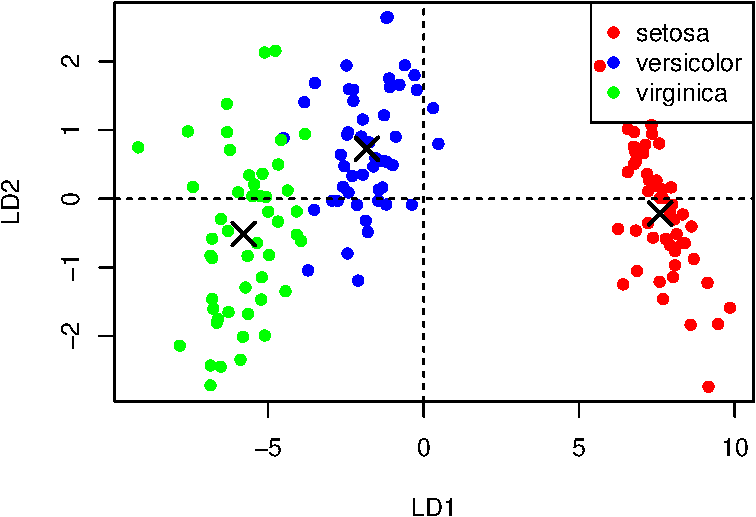
\includegraphics{lista-3_files/figure-pdf/fig-ldairis-1.pdf}

}

\caption{\label{fig-ldairis}Gráfico de Classificação do LDA para o
Conjunto de Dados Iris}

\end{figure}%

\newpage{}

\section{Questão 10 - Critério de Minimos
Quadrados}\label{questuxe3o-10---crituxe9rio-de-minimos-quadrados}

No R, a utilização do critério de Mínimos Quadrados pode ser
exemplificada por meio de regressão linear e modelos lineares
generalizados, utilizando as funções lm() e glm(), respectivamente. A
implementação deste critério no R oferece várias vantagens, incluindo
uma ampla gama de funções que o utilizam como base, facilidade de uso
devido à sintaxe intuitiva e uma vasta comunidade que compartilha
informações e recursos sobre essas implementações. Contudo, assim como o
critério de Fisher, o critério de Mínimos Quadrados enfrenta desafios,
como dificuldade em lidar com conjuntos de dados muito grandes, questões
de desempenho e limitações de memória computacional .

\subsection{Exemplo}\label{exemplo-4}

Vamos aplicar uma regressão logística usando o pacote stats.
Primeiramente, ajustaremos uma regressão linear simples com \(x_1\) e
\(x_2\) sendo variáveis simuladas de uma distribuição normal com médias
2 e 3, respectivamente, e \(y\) sendo uma combinação de \(x_1\) e
\(x_2\) com uma distribuição normal de média 0, posteriormente
transformada em uma variável binária. Embora este problema seja mais
adequado para uma regressão logística, usaremos este exemplo para
ilustrar o critério de Mínimos Quadrados.

\begin{Shaded}
\begin{Highlighting}[]
\CommentTok{\# Gerar dados de exemplo}
\FunctionTok{set.seed}\NormalTok{(}\DecValTok{123}\NormalTok{)}
\NormalTok{n }\OtherTok{\textless{}{-}} \DecValTok{100}
\NormalTok{x1 }\OtherTok{\textless{}{-}} \FunctionTok{rnorm}\NormalTok{(n, }\AttributeTok{mean =} \DecValTok{2}\NormalTok{, }\AttributeTok{sd =} \DecValTok{1}\NormalTok{)}
\NormalTok{x2 }\OtherTok{\textless{}{-}} \FunctionTok{rnorm}\NormalTok{(n, }\AttributeTok{mean =} \DecValTok{3}\NormalTok{, }\AttributeTok{sd =} \DecValTok{1}\NormalTok{)}
\NormalTok{y }\OtherTok{\textless{}{-}} \FunctionTok{ifelse}\NormalTok{(x1 }\SpecialCharTok{+}\NormalTok{ x2 }\SpecialCharTok{+} \FunctionTok{rnorm}\NormalTok{(n) }\SpecialCharTok{\textgreater{}} \DecValTok{5}\NormalTok{, }\DecValTok{1}\NormalTok{, }\DecValTok{0}\NormalTok{)}
\NormalTok{dados }\OtherTok{\textless{}{-}} \FunctionTok{data.frame}\NormalTok{(x1, x2, y)}

\CommentTok{\# Ajustar o modelo de regressão linear}
\NormalTok{modelo\_linear }\OtherTok{\textless{}{-}} \FunctionTok{lm}\NormalTok{(y }\SpecialCharTok{\textasciitilde{}}\NormalTok{ x1 }\SpecialCharTok{+}\NormalTok{ x2, }\AttributeTok{data =}\NormalTok{ dados)}
\FunctionTok{summary}\NormalTok{(modelo\_linear)}
\end{Highlighting}
\end{Shaded}

\begin{verbatim}

Call:
lm(formula = y ~ x1 + x2, data = dados)

Residuals:
     Min       1Q   Median       3Q      Max 
-0.66422 -0.32225 -0.02538  0.25805  0.84446 

Coefficients:
            Estimate Std. Error t value Pr(>|t|)    
(Intercept) -0.73012    0.15228  -4.794 5.89e-06 ***
x1           0.19884    0.04189   4.746 7.14e-06 ***
x2           0.29541    0.03955   7.470 3.53e-11 ***
---
Signif. codes:  0 '***' 0.001 '**' 0.01 '*' 0.05 '.' 0.1 ' ' 1

Residual standard error: 0.38 on 97 degrees of freedom
Multiple R-squared:  0.436, Adjusted R-squared:  0.4244 
F-statistic:  37.5 on 2 and 97 DF,  p-value: 8.616e-13
\end{verbatim}

\begin{Shaded}
\begin{Highlighting}[]
\CommentTok{\# Fazer previsões}
\NormalTok{probabilidades }\OtherTok{\textless{}{-}} \FunctionTok{predict}\NormalTok{(modelo\_linear,}\AttributeTok{newdata =}\NormalTok{ dados, }\AttributeTok{type =} \StringTok{"response"}\NormalTok{)}

\CommentTok{\# Transformar as probabilidades em classes binárias}
\NormalTok{predicoes }\OtherTok{\textless{}{-}} \FunctionTok{ifelse}\NormalTok{(probabilidades }\SpecialCharTok{\textgreater{}} \FloatTok{0.7}\NormalTok{, }\DecValTok{1}\NormalTok{, }\DecValTok{0}\NormalTok{)}

\CommentTok{\# Avaliar a precisão}
\NormalTok{precisao }\OtherTok{\textless{}{-}} \FunctionTok{mean}\NormalTok{(predicoes }\SpecialCharTok{==}\NormalTok{ dados}\SpecialCharTok{$}\NormalTok{y)}
\end{Highlighting}
\end{Shaded}

Assim calculamos a precisão comparando as previsões com as classes
verdadeiras, obtendo um grau de precisão de 0.79.

\newpage{}

\section*{Referências}\label{referuxeancias}
\addcontentsline{toc}{section}{Referências}

\phantomsection\label{refs}
\begin{CSLReferences}{1}{0}
\bibitem[\citeproctext]{ref-curtin2017designing}
Curtin, Ryan R, e Marcus Edel. 2017. {«Designing and building the mlpack
open-source machine learning library»}. \emph{arXiv preprint
arXiv:1708.05279}.

\bibitem[\citeproctext]{ref-edel2014automatic}
Edel, Marcus, Anand Soni, e Ryan R Curtin. 2014. {«An automatic
benchmarking system»}. Em \emph{NIPS 2014 Workshop on Software
Engineering for Machine Learning}.

\end{CSLReferences}



\end{document}
